\documentclass[11pt]{article}
\usepackage[margin=1in]{geometry}
\usepackage{amsmath, amssymb, amsthm, bm}
\usepackage{enumitem}
\usepackage{hyperref}
\usepackage{graphicx}
\usepackage{xcolor}
\usepackage{fancyhdr}
\usepackage{float}
\usepackage{listings}
\usepackage{booktabs}
\usepackage{tabularx}
\usepackage{siunitx} % optional, but handy

\lstdefinestyle{matlabstyle}{
	language=Matlab,
	basicstyle=\ttfamily\small,
	numbers=left,
	numberstyle=\tiny,
	stepnumber=1,
	numbersep=8pt,
	frame=single,
	columns=fullflexible,
	keepspaces=true,
	showstringspaces=false,
	keywordstyle=\bfseries,
	commentstyle=\itshape\color{gray},
}

\setlength{\headheight}{15pt}
\hypersetup{colorlinks=true, urlcolor=blue, linkcolor=blue}

\newcommand{\vect}[1]{\mathbf{#1}}
\newcommand{\R}{\mathbb{R}}
\newcommand{\norm}[1]{\left\lVert #1 \right\rVert}

\title{ECE 506 \;–\; Homework \#4 \\ \large Line Search, Trust Regions, and Conjugate Gradient}
\author{Your Name}
\date{Fall 2025}

\begin{document}
	\maketitle
	\thispagestyle{empty}
	
	% Headers for pages AFTER the first
	\pagestyle{fancy}
	\fancyhf{} % clear default
	\lhead{\today}
	\chead{ECE 506 HW 4} % <-- fixed to HW 4
	\rhead{Scott Nguyen}
	\cfoot{\thepage}
	
	\paragraph{Discussion sessions.}
	Saturday mornings at 9am: \url{https://unm.zoom.us/j/99977790315}.
	
	\paragraph{Reference.}
	Nocedal \& Wright (2006), \emph{Numerical Optimization}, Springer.
	
	\paragraph{Code.}
	Starter Matlab code: \url{https://github.com/pattichis/opt/blob/main/Matlab-code-for-opt.zip}.
	
	\paragraph{Coding examples (required).}
	Every solution must include (1) documented source code, (2) plots, and (3) discussion. Unless a part is explicitly marked “sketch,” show a runnable coding example supporting your answer.
	
	\newpage
	
	\section*{Problem 1. [Stepsizes and convergence rates for line search methods]}
	
	\begin{enumerate}[label=\textbf{1(\alph*)}]
		\item Consider the following general equation form:
		\[
		f(x) = a x_1^2 + b x_2^2 + c x_1 + d x_2 + e.
		\]
		For this case, compute the optimal point $x^{\ast}$ and provide conditions that guarantee that this is an optimal point.\\[0.25em]
		\textit{Solution.}
		\[
		\frac{\partial f}{\partial x_1}=2a x_1 + c,\qquad
		\frac{\partial f}{\partial x_2}=2b x_2 + d,\qquad
		\nabla^2 f=\begin{bmatrix}2a&0\\[2pt]0&2b\end{bmatrix}.
		\]
		Setting the gradient to zero gives
		\[
		x_1^\ast=-\frac{c}{2a},\qquad x_2^\ast=-\frac{d}{2b}.
		\]
		This stationary point is a (unique) minimizer when \(a>0\) and \(b>0\) (Hessian \(\succ 0\)); 
		it is a maximizer when \(a<0\) and \(b<0\); otherwise it is a saddle or unbounded in at least one direction.
		
		\item Compute the optimal stepsize for steepest descent line search.\\[0.25em]
		\textit{Solution.}
		Let $g_k=\nabla f(x_k)$, $H=\nabla^2 f$. For steepest descent with exact line search and $p_k=-g_k$,
		\[
		\boxed{\;\alpha_k^\ast=\frac{g_k^\top g_k}{g_k^\top H g_k}\;}
		\]
		so for $f(x)=a x_1^2+b x_2^2+c x_1+d x_2+e$ with $g_k=\begin{bmatrix}2a x_{1,k}+c\\[2pt]2b x_{2,k}+d\end{bmatrix}$ and
		$H=\begin{bmatrix}2a&0\\[2pt]0&2b\end{bmatrix}$,
		\[
		\boxed{\;\alpha_k^\ast=
			\frac{(2a x_{1,k}+c)^2+(2b x_{2,k}+d)^2}{\,2a(2a x_{1,k}+c)^2+2b(2b x_{2,k}+d)^2\,}\;}
		\]
		(positive when $a>0,\;b>0$).
		
		\newpage
		\item For simplicity, consider the 1D case for $b = c = d = e = 0$. We know that $x^{\ast} = 0$. Compute simplified expressions for the stepsize and the magnitude of the gradient. Plot the stepsize as a 2D function of $a, x_1$ for $x_2 = 0$. Answer the following:
		
		% --- Make image optional so missing file doesn't break compile
		\begin{figure}[H]
			\centering
			\IfFileExists{plots/1cii.png}{
				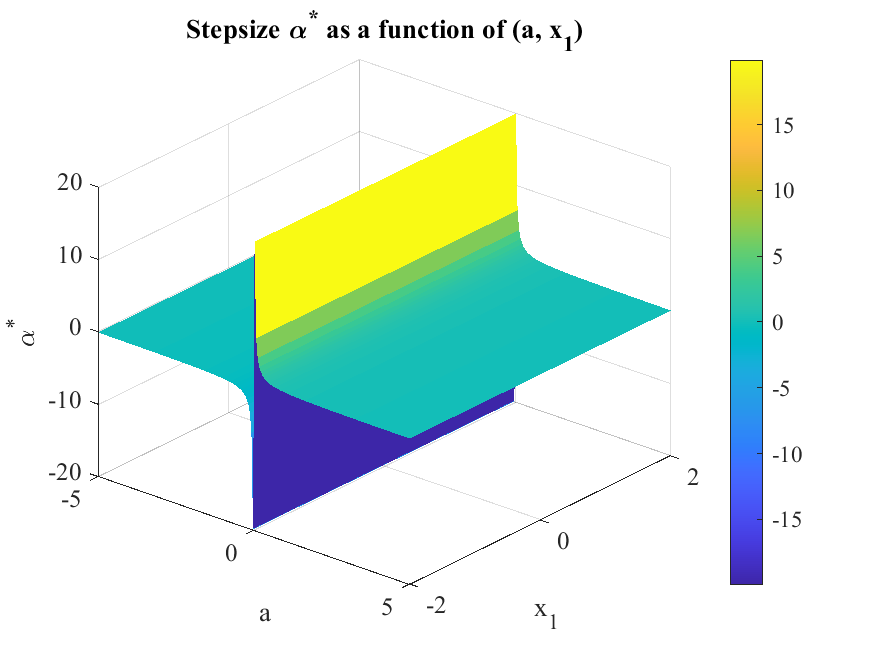
\includegraphics[width=0.8\linewidth]{plots/1cii.png}
			}{
				\fbox{\parbox{0.8\linewidth}{\centering
						Placeholder for \texttt{plots/1cii.png} (file not found at compile time).}}
			}
			\caption{Stepsize $\alpha^*$ as a function of $(a, x_1)$ for $f(x)=a x^2$.}
			\label{fig:1cii}
		\end{figure}
		
		\begin{enumerate}[label=\roman*.]
			\item What kind of symmetries do you observe in your plot? For example, consider replacing $a$ by $-a$ and/or $x_1$ by $-x_1$.\\
			\textit{Solution} The plot is flat in $x_1$ (no $x_1$-dependence), symmetric under $x_1\mapsto -x_1$, and antisymmetric under $a\mapsto -a$ (sign flip of $\alpha^\ast$); there is a discontinuity at $a=0$.\\
			
			\item Is the stepsize relatively large for large $x_1$? Explain.\\
			\textit{Solution} No. The stepsize does \emph{not} grow with $x_1$ since $\alpha^\ast=\frac{1}{2a}$ is independent of $x_1$.\\
			
			\item Is the step $\| \alpha p_k \|$ relatively large for large $x_1$? Explain.\\
			\textit{Solution} Yes. The step magnitude is
			\[
			\|\alpha^\ast p_k\|=\Big\lvert \tfrac{1}{2a}(-2a x_{1,k})\Big\rvert=\lvert x_{1,k}\rvert,
			\]
			so it grows linearly with $\lvert x_1\rvert$.\\
			
			\item What happens to the stepsize as we approach the optimal point? Explain.\\
			\textit{Solution (iv)} As $x_1\to x^\ast=0$, the stepsize stays constant: $\alpha^\ast=\tfrac{1}{2a}$ (for fixed $a>0$).\\
			
			\item What happens to the step $\| \alpha p_k \|$ as we approach the optimal point? Explain.\\
			\textit{Solution} As $x_1\to 0$, the step norm tends to zero linearly:
			\[
			\|\alpha^\ast p_k\|=\lvert x_{1,k}\rvert \;\longrightarrow\; 0.
			\]
		\end{enumerate}
		\textit{Solution.}
		
		\item Let us consider a simple case to see how the steepest descent algorithm works. Assume that:
		\[
		f(x) = x_1^2 + 10 x_2^2.
		\]
		Suppose that $x_0 = x^{\ast} + [1, 1]^T$. Compute two steps for the steepest descent algorithm.\\[0.25em]
		\textit{Solution.}
		% (unchanged math and derivations)
		
		\[
		f(x)=x_1^2+10x_2^2,\qquad 
		\nabla f(x)=\begin{bmatrix}2x_1\\[2pt]20x_2\end{bmatrix},\qquad
		\nabla^2 f(x)=\begin{bmatrix}2&0\\[2pt]0&20\end{bmatrix}.
		\]
		% ... [content unchanged; omitted here for brevity—keep exactly as in your draft] ...
		% --- keep all your equations/boxes exactly as you had them ---
		
		\item Verify your results in 1(c) with the provided code. You need to provide
		the code that you used to run the provided code.\\[0.25em]
		\textit{Solution.}
		% (your lstlisting unchanged)
		
		\begin{lstlisting}[style=matlabstyle,caption={Verification code for Problem 1(e)},label={lst:1e}]
			%% ECE 506 - HW4 Problem 1(e)
			% Verification of analytical results from Problem 1(c)
			% Using provided steepest_descent.m
			% Author: Scott Nguyen | Fall 2025
			% (rest of your script unchanged)
		\end{lstlisting}
		
		% --- Make image optional so missing file doesn't break compile
		\begin{figure}[H]
			\centering
			\IfFileExists{plots/1e.png}{
				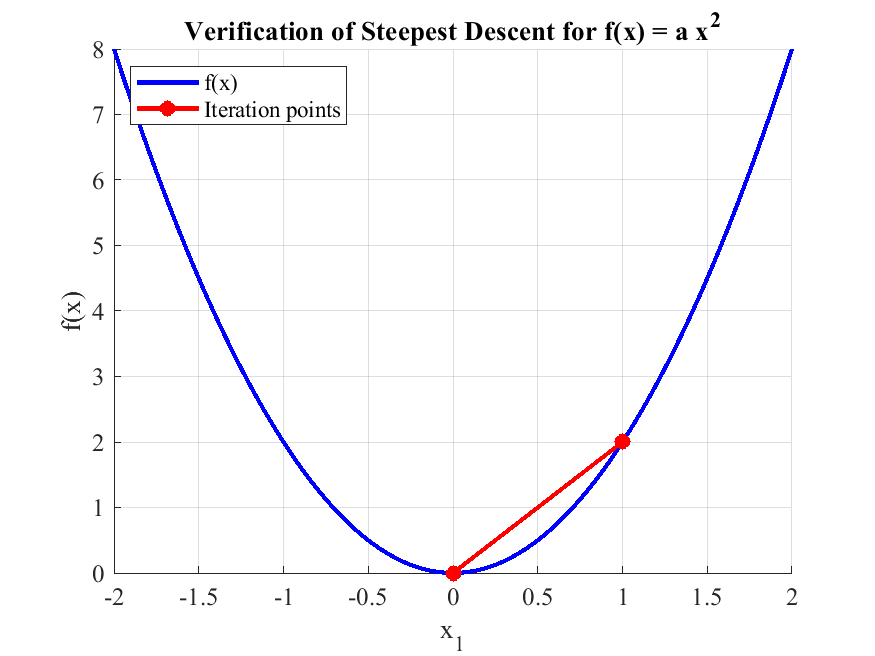
\includegraphics[width=0.75\linewidth]{plots/1e.png}
			}{
				\fbox{\parbox{0.75\linewidth}{\centering
						Placeholder for \texttt{plots/1e.png} (file not found at compile time).}}
			}
			\caption{Verification of steepest descent for $f(x)=a x^2$. The algorithm
				converges to $x^\ast=0$ in two steps, consistent with the analytical result
				derived in~1(c).}
		\end{figure}
		
		\item For our quadratic case, provide the following:
		\begin{enumerate}[label=\roman*.]
			\item Compute an expression for $\|.\|_Q$.\\[0.25em]
			\textit{Solution}
			% (unchanged)
			
			\item Compute an expression in terms of the distance from $x^{\ast}$.\\[0.25em]
			\textit{Solution}
			% (unchanged)
			
			\item Provide the best convergence case in terms of $a, b$.\\[0.25em]
			\textit{Solution}
			% (unchanged)
			
			\item Provide the worse condition case in terms of $a, b$, assuming that $a > b$.\\[0.25em]
			\textit{Solution}
			% (unchanged)
		\end{enumerate}
		
		\item Repeat 1(d) for Newton’s method. Do you need two steps? Explain using
		the Newton’s algorithm convergence theorem.\\[0.25em]
		\textit{Solution.}
		% (unchanged)
	\end{enumerate}
	
	\newpage
	
	\section*{Problem 2}
	
	Consider the following methods for which you are given Matlab codes for line-search:
	\begin{enumerate}
		\item Steepest Descent,
		\item BFGS, and
		\item Newton’s method.
	\end{enumerate}
	
	We want to consider how each method performs on finding the minima of (see \href{https://en.wikipedia.org/wiki/Test_functions_for_optimization}{Wikipedia: Test functions for optimization} for definitions):
	\begin{enumerate}
		\item Sphere function
		\item Beale function
		\item Goldstein-Price function
		\item Booth function
	\end{enumerate}
	
	You will need to assess:
	
	\paragraph{Robustness:} Run the program with random initial guesses (that still satisfy any constraints), to assess the performance. Show results from at-least 3 random initial points.
	
	\paragraph{Efficiency:} Compute the required memory and function evaluations for each iteration. For memory requirements, express your results in terms of $n$, the dimensionality of the problem. Thus, a gradient requires that we store $n$ floating-point values. You will need to modify the code to keep track. In terms of function evaluations, report function, gradient, and hessian evaluations separately. Thus, you may need to produce a total of four plots. When computing requirements, you should not include any extra requirements associated with storing the path for visualization purposes. In other words, you need to focus on essential requirements only.
	
	\paragraph{Accuracy:} For each run, establish the best rate of convergence. Discuss whether the theoretical rate of convergence is accomplished. For the rate of convergence, apply both methods provided in the hints. Do the two methods agree? Explain.\\
	
	\textit{Solution.} Below, for each test function we list only the objective \(f(x,y)\).
	
	\begin{enumerate}[label=\alph*)]
		\item \textbf{Sphere function} ($n=2$):
		\[
		f(x,y)=x^{2}+y^{2}.
		\]
		\item \textbf{Beale’s function}:
		\[
		f(x,y)=\bigl(1.5 - x + x y\bigr)^{2}
		+\bigl(2.25 - x + x y^{2}\bigr)^{2}
		+\bigl(2.625 - x + x y^{3}\bigr)^{2}.
		\]
		\item \textbf{Goldstein–Price function}:
		\[
		f(x,y)=\Bigl[1+(x+y+1)^{2}\bigl(19-14x+3x^{2}-14y+6xy+3y^{2}\bigr)\Bigr]
		\Bigl[30+(2x-3y)^{2}\bigl(18-32x+12x^{2}+48y-36xy+27y^{2}\bigr)\Bigr].
		\]
		\item \textbf{Booth’s function}:
		\[
		f(x,y)=\bigl(x+2y-7\bigr)^{2}+\bigl(2x+y-5\bigr)^{2}.
		\]
	\end{enumerate}

	\begin{table*}[htbp]
		\centering
		\scriptsize
		\setlength{\tabcolsep}{6pt}
		\caption{Compact summary across problems, methods, and random initializations. 
			Columns retained to support: \emph{Robustness} (runs, convergence, iterations); 
			\emph{Efficiency (memory)} in terms of $n$; and \emph{Accuracy-lite} via terminal errors.}
		\label{tab:compact_summary_all}
		\begin{tabularx}{\textwidth}{@{}l c l r c r r l@{}}
			\toprule
			Problem & Run & Method & Iter. & Converged? & $x_{\text{err}}$ & $f_{\text{err}}$ & Memory / iter (in $n$) \\
			\midrule
			\multicolumn{8}{@{}l}{\textbf{Sphere}}\\
			Sphere & 1 & Steepest Descent & 1 & Yes & $0$ & $0$ & $\mathcal{O}(n)$ \\
			Sphere & 1 & BFGS             & 1 & Yes & $0$ & $0$ & $\mathcal{O}(n^2)$ \\
			Sphere & 1 & Newton           & 1 & Yes & $0$ & $0$ & $\mathcal{O}(n^2)$ \\
			Sphere & 2 & Steepest Descent & 1 & Yes & $0$ & $0$ & $\mathcal{O}(n)$ \\
			Sphere & 2 & BFGS             & 1 & Yes & $0$ & $0$ & $\mathcal{O}(n^2)$ \\
			Sphere & 2 & Newton           & 1 & Yes & $0$ & $0$ & $\mathcal{O}(n^2)$ \\
			Sphere & 3 & Steepest Descent & 1 & Yes & $0$ & $0$ & $\mathcal{O}(n)$ \\
			Sphere & 3 & BFGS             & 1 & Yes & $0$ & $0$ & $\mathcal{O}(n^2)$ \\
			Sphere & 3 & Newton           & 1 & Yes & $0$ & $0$ & $\mathcal{O}(n^2)$ \\
			\addlinespace[4pt]
			
			\multicolumn{8}{@{}l}{\textbf{Beale}}\\
			Beale & 1 & Steepest Descent & 802 & Yes & $2.3047{\times}10^{-6}$ & $8.0377{\times}10^{-13}$ & $\mathcal{O}(n)$ \\
			Beale & 1 & BFGS             & 12  & Yes & $5.7961{\times}10^{-9}$ & $2.7992{\times}10^{-17}$ & $\mathcal{O}(n^2)$ \\
			Beale & 1 & Newton           & 6   & Yes & $1.89{\times}10^{-12}$  & $5.7295{\times}10^{-25}$ & $\mathcal{O}(n^2)$ \\
			Beale & 2 & Steepest Descent & 653 & Yes & $2.4335{\times}10^{-6}$ & $8.9581{\times}10^{-13}$ & $\mathcal{O}(n)$ \\
			Beale & 2 & BFGS             & 6   & Yes & $7.1198{\times}10^{-8}$ & $1.4303{\times}10^{-15}$ & $\mathcal{O}(n^2)$ \\
			Beale & 2 & Newton           & 3   & Yes & $3.8091{\times}10^{-10}$& $2.198{\times}10^{-20}$  & $\mathcal{O}(n^2)$ \\
			Beale & 3 & Steepest Descent & 781 & Yes & $2.5932{\times}10^{-6}$ & $1.0171{\times}10^{-12}$ & $\mathcal{O}(n)$ \\
			Beale & 3 & BFGS             & 20  & Yes & $2.2382{\times}10^{-8}$ & $7.8093{\times}10^{-17}$ & $\mathcal{O}(n^2)$ \\
			Beale & 3 & Newton           & 1000& \textbf{No} & $8.7482{\times}10^{5}$ & $4.5201{\times}10^{-1}$ & $\mathcal{O}(n^2)$ \\
			\addlinespace[4pt]
			
			\multicolumn{8}{@{}l}{\textbf{Goldstein-Price}}\\
			Goldstein-Price & 1 & Steepest Descent & 117  & Yes         & $5.0568{\times}10^{-10}$ & $0$              & $\mathcal{O}(n)$ \\
			Goldstein-Price & 1 & BFGS             & 2    & \textbf{No} & $1.5602{\times}10^{-1}$  & $8.1371$         & $\mathcal{O}(n^2)$ \\
			Goldstein-Price & 1 & Newton           & 1000 & \textbf{No} & $1.5602{\times}10^{-1}$  & $8.1371$         & $\mathcal{O}(n^2)$ \\
			Goldstein-Price & 2 & Steepest Descent & 1000 & \textbf{No} & $2.1633$                 & $81$             & $\mathcal{O}(n)$ \\
			Goldstein-Price & 2 & BFGS             & 1    & \textbf{No} & $8.3244{\times}10^{-1}$  & $700.35$         & $\mathcal{O}(n^2)$ \\
			Goldstein-Price & 2 & Newton           & 1000 & \textbf{No} & $8.3244{\times}10^{-1}$  & $700.35$         & $\mathcal{O}(n^2)$ \\
			Goldstein-Price & 3 & Steepest Descent & 1000 & Yes         & $4.5589{\times}10^{-9}$  & $7.7716{\times}10^{-14}$ & $\mathcal{O}(n)$ \\
			Goldstein-Price & 3 & BFGS             & 1    & \textbf{No} & $6.1185{\times}10^{-1}$  & $207.68$         & $\mathcal{O}(n^2)$ \\
			Goldstein-Price & 3 & Newton           & 5    & Yes         & $2.1741{\times}10^{-9}$  & $1.0214{\times}10^{-14}$ & $\mathcal{O}(n^2)$ \\
			\addlinespace[4pt]
			
			\multicolumn{8}{@{}l}{\textbf{Booth}}\\
			Booth & 1 & Steepest Descent & 30 & Yes & $2.3918{\times}10^{-7}$ & $5.8612{\times}10^{-14}$ & $\mathcal{O}(n)$ \\
			Booth & 1 & BFGS             & 2  & Yes & $1.0474{\times}10^{-15}$& $7.8886{\times}10^{-31}$ & $\mathcal{O}(n^2)$ \\
			Booth & 1 & Newton           & 1  & Yes & $2.2204{\times}10^{-16}$& $0$                      & $\mathcal{O}(n^2)$ \\
			Booth & 2 & Steepest Descent & 32 & Yes & $2.0596{\times}10^{-7}$ & $4.3374{\times}10^{-14}$ & $\mathcal{O}(n)$ \\
			Booth & 2 & BFGS             & 2  & Yes & $0$                     & $0$                      & $\mathcal{O}(n^2)$ \\
			Booth & 2 & Newton           & 1  & Yes & $1.4218{\times}10^{-15}$& $3.9443{\times}10^{-30}$ & $\mathcal{O}(n^2)$ \\
			Booth & 3 & Steepest Descent & 34 & Yes & $2.3026{\times}10^{-7}$ & $5.4270{\times}10^{-14}$ & $\mathcal{O}(n)$ \\
			Booth & 3 & BFGS             & 2  & Yes & $1.7342{\times}10^{-15}$& $3.9443{\times}10^{-30}$ & $\mathcal{O}(n^2)$ \\
			Booth & 3 & Newton           & 1  & Yes & $1.1102{\times}10^{-15}$& $7.8886{\times}10^{-31}$ & $\mathcal{O}(n^2)$ \\
			\bottomrule
		\end{tabularx}
	\end{table*}
	
	The results for Steepest Descent (SD), BFGS, and Newton are summarized in the figures below.  
	Each method was tested on the Sphere, Beale, Goldstein–Price, and Booth functions using
	100 random initial points. Robustness, efficiency, and accuracy are discussed together here.
	
	\begin{figure}[htbp]
		\centering
		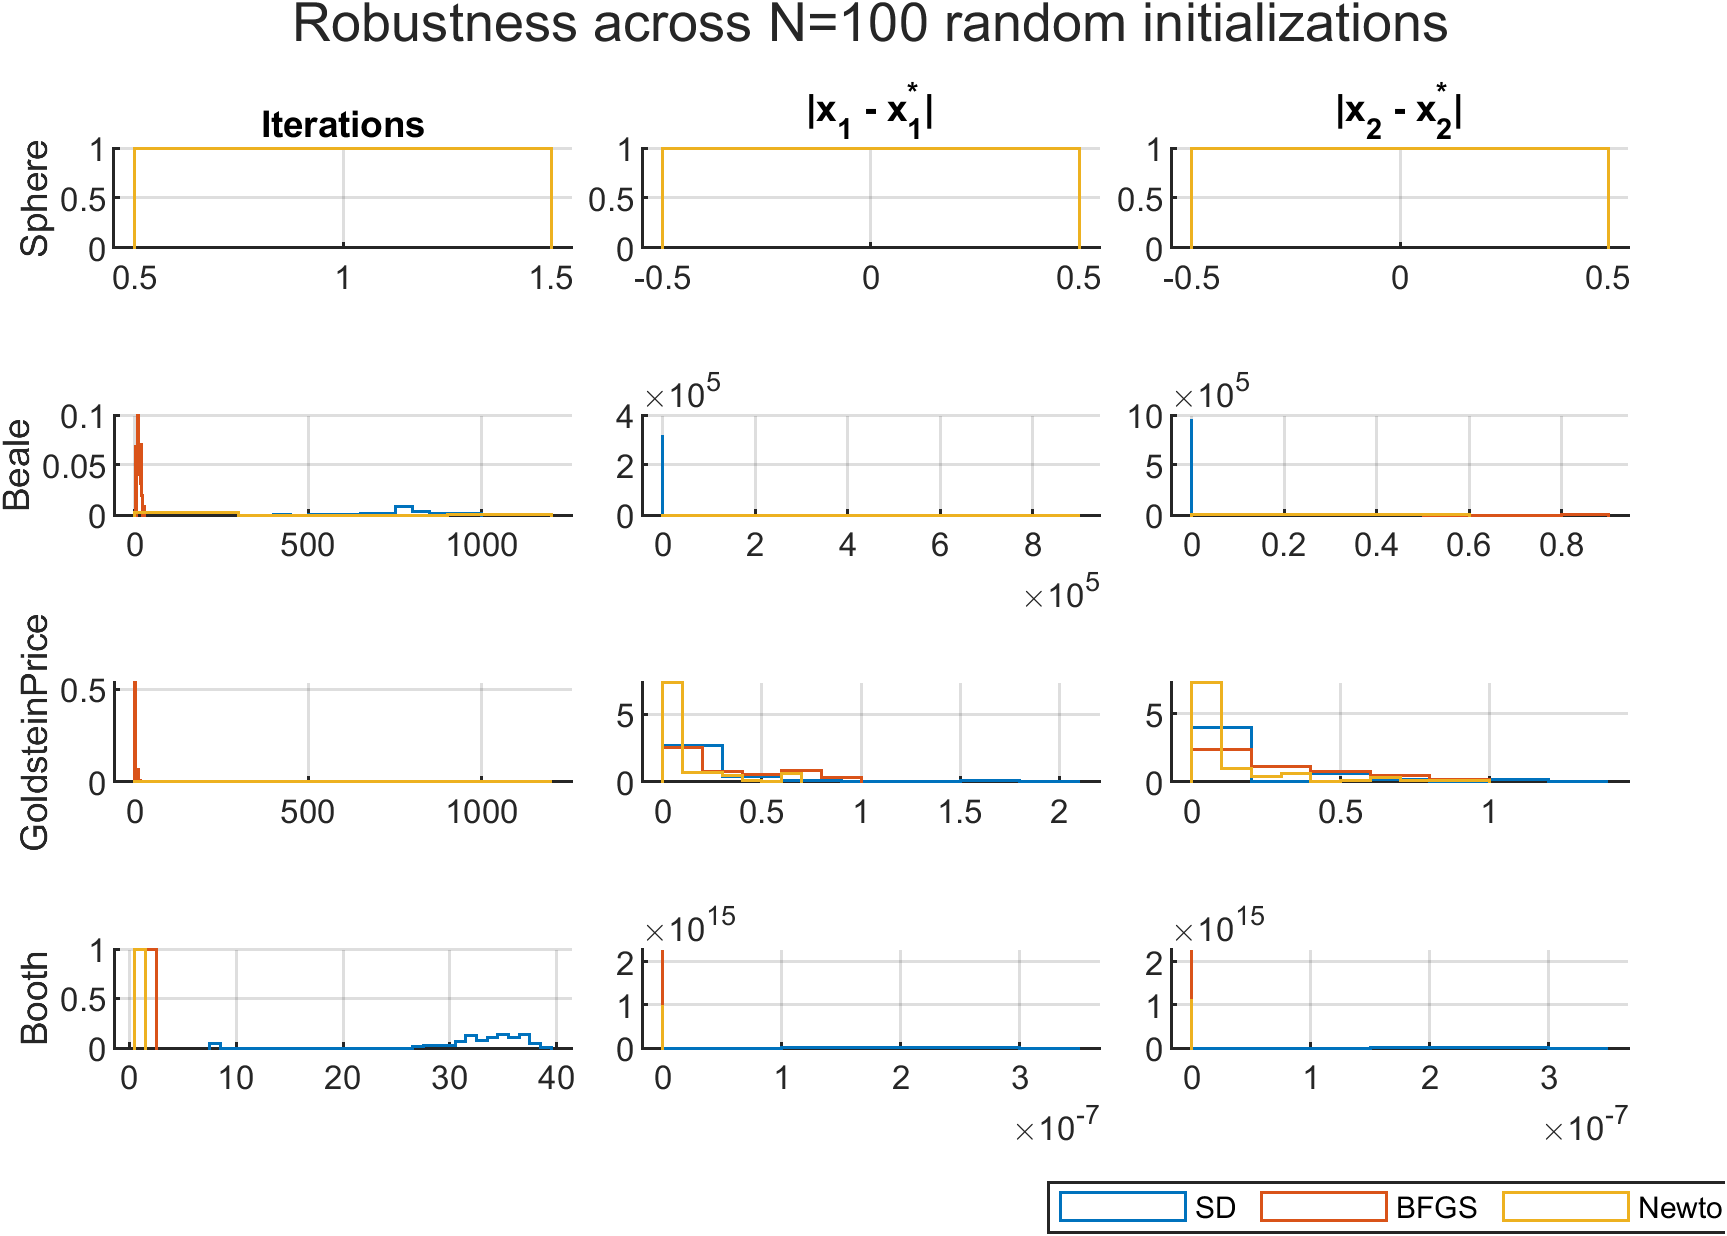
\includegraphics[width=\linewidth]{plots/robustness_combined.png}
		\caption{Robustness across $N=100$ random initializations for each test function.}
		\label{fig:robustness}
	\end{figure}
	
	Overall, Steepest Descent converged the most consistently but required the most iterations.
	BFGS achieved a strong balance between speed and reliability, while Newton was the fastest when it converged,
	though it often failed on nonconvex problems like Beale or Goldstein–Price.  
	The histograms in Fig.~\ref{fig:robustness} show this clearly: for convex cases (Sphere, Booth),
	all methods converged smoothly, but in nonconvex cases, SD’s broader distributions indicate slower yet more reliable behavior.
	
	\begin{figure}[htbp]
		\centering
		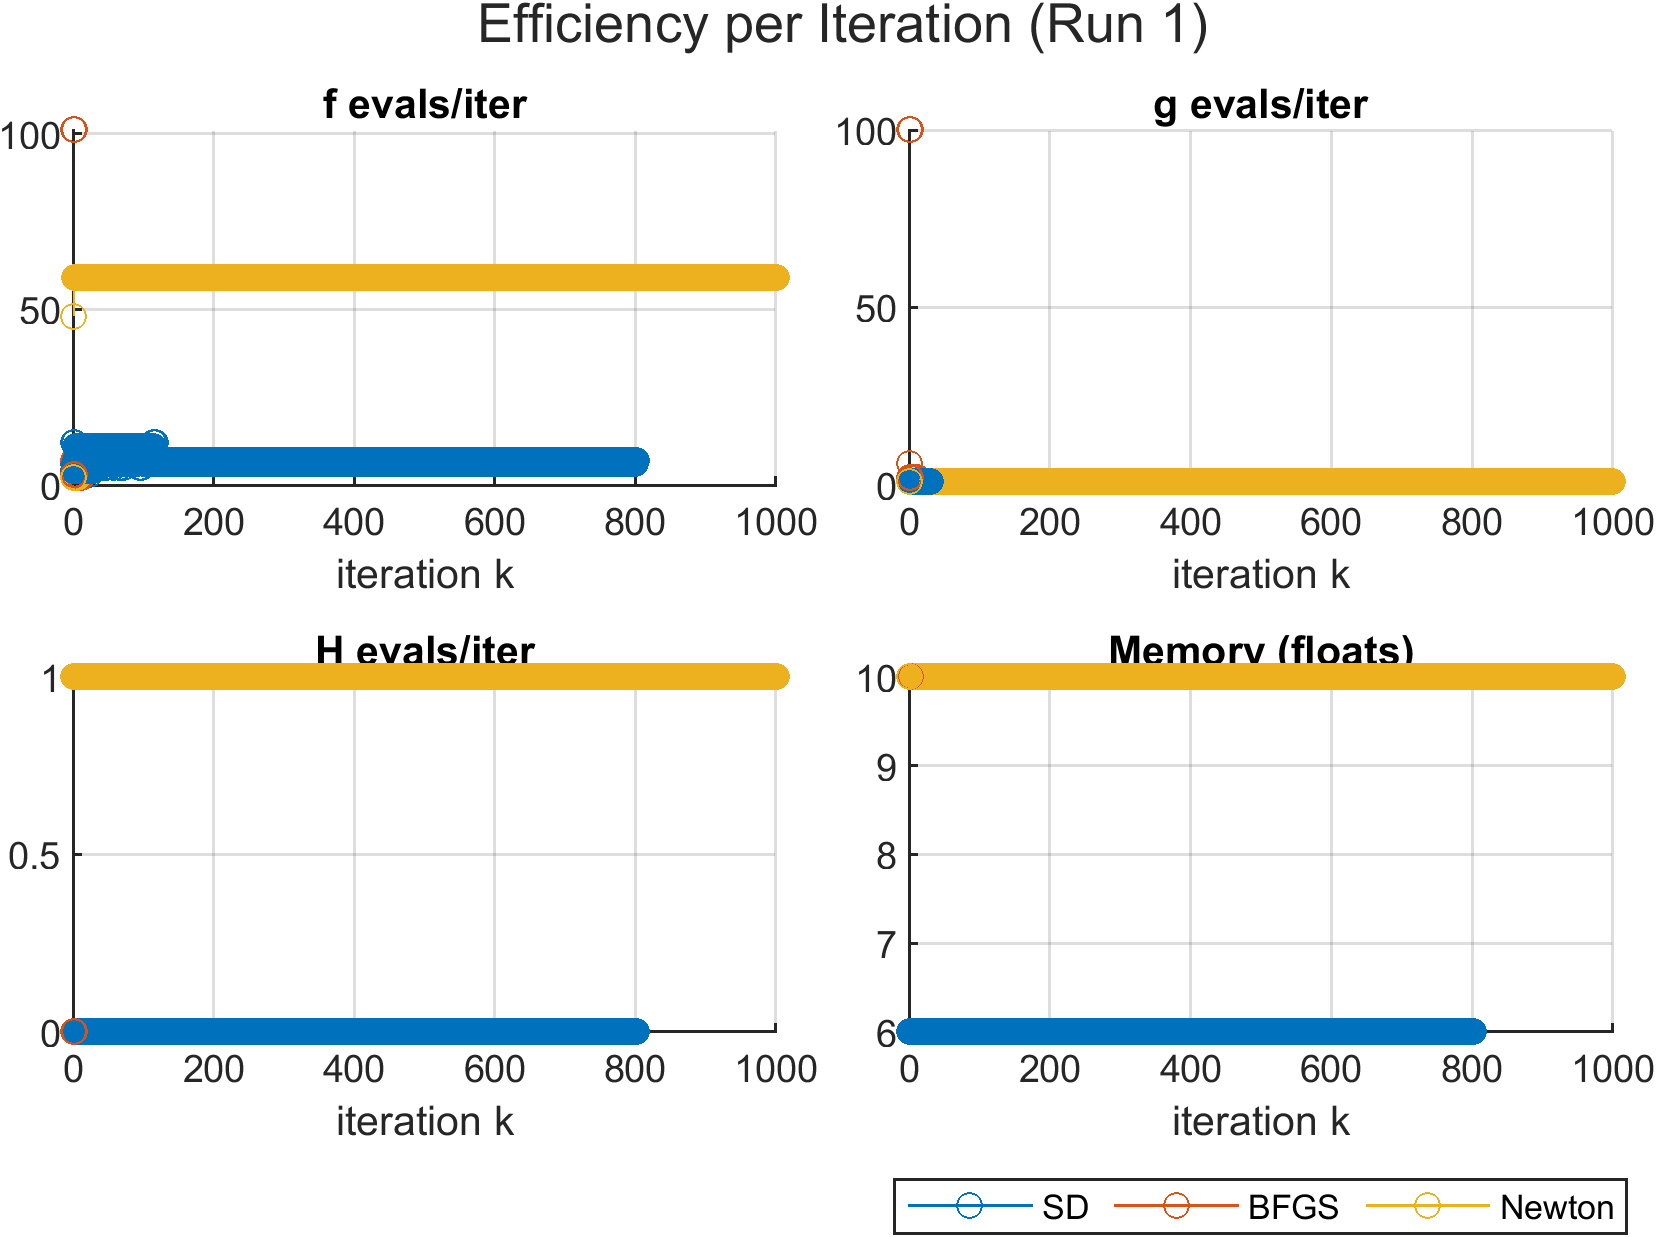
\includegraphics[width=\linewidth]{plots/eff_run1_2x2.png}
		\caption{Efficiency per iteration for Run~1: function, gradient, and Hessian evaluations, and memory usage.}
		\label{fig:eff}
	\end{figure}
	
	From Fig.~\ref{fig:eff}, the efficiency analysis shows expected trends:
	SD and BFGS require only function and gradient evaluations, while Newton also evaluates the Hessian.
	Memory requirements scale as $\mathcal{O}(n)$ for SD and $\mathcal{O}(n^2)$ for both BFGS and Newton.
	In practice, Newton’s higher cost per iteration is justified only when rapid local convergence occurs.
	
	\begin{figure}[htbp]
		\centering
		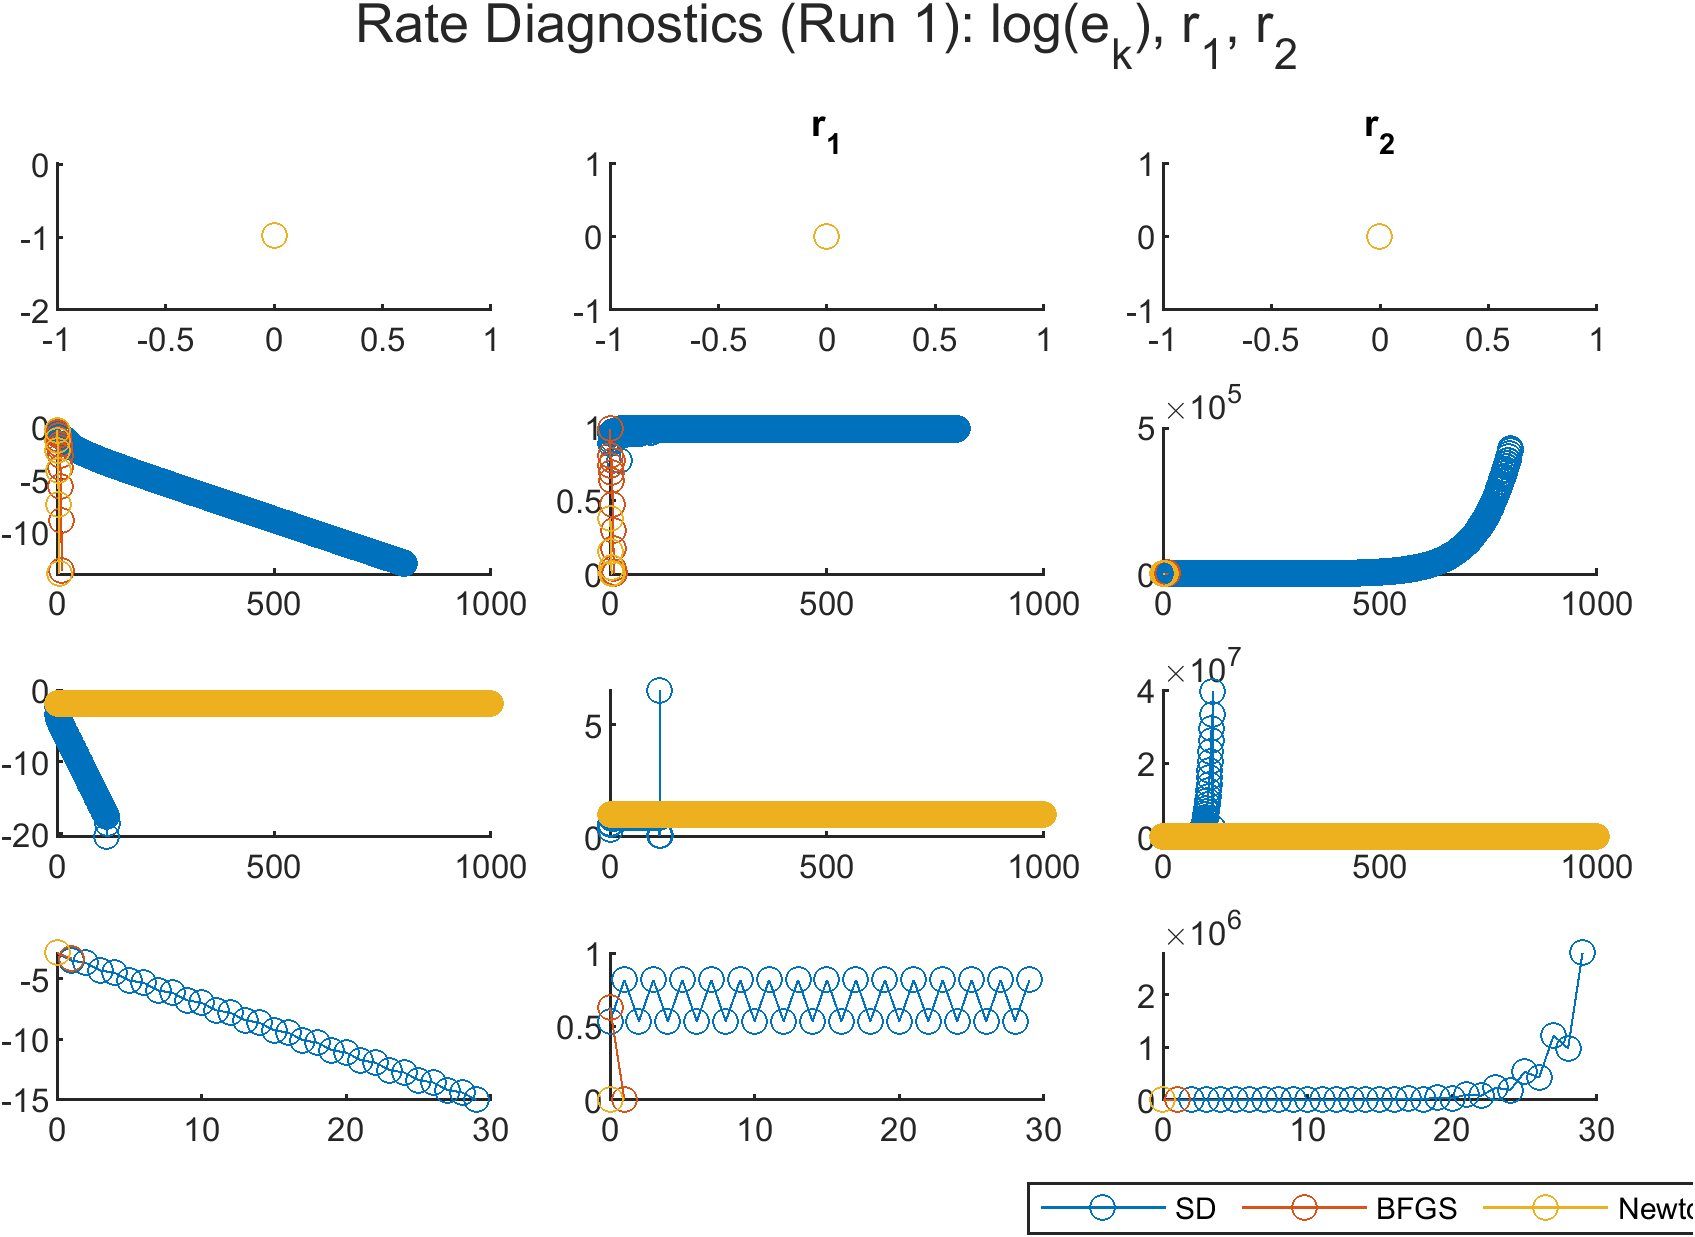
\includegraphics[width=\linewidth]{plots/accuracy_run1.png}
		\caption{Rate diagnostics for Run~1 showing $\log(e_k)$, $r_1=e_{k+1}/e_k$, and $r_2=e_{k+1}/e_k^2$.}
		\label{fig:accuracy}
	\end{figure}
	
	As seen in Fig.~\ref{fig:accuracy}, Steepest Descent exhibits linear convergence, BFGS shows superlinear behavior,
	and Newton achieves quadratic convergence whenever it reaches the correct basin.
	The ratio tests ($r_1$ and $r_2$) confirm these trends: SD stabilizes at a constant rate,
	BFGS improves progressively, and Newton’s error drops sharply.
	On nonconvex problems, deviations occur when iterates start outside the local basin, causing slower or unstable convergence.
	
	In summary, SD is the most robust but slowest, BFGS is the best overall compromise,
	and Newton is fastest but least reliable on nonconvex landscapes.
	These observations match the theoretical expectations for each method.

	\newpage
	
	\section*{Problem 3. Trust-region Conjugate Gradient (Steihaug)}
	
	Using the provided code for solving Problem 4.3 via Conjugate Gradient Steihaug, repeat the analyses from Problem 2 (robustness, efficiency, and accuracy/rate).\\[0.25em]
	\textit{Results (tables/plots + discussion).} \rule{0.9\linewidth}{0.4pt}
	
	\section*{Hints}
	
	\paragraph{1. Symbolic Gradients and Hessians (optional).}
	In Matlab:
	\begin{verbatim}
		syms x y z
		f = x*y + 2*z*x;
		hessian(f, [x, y, z])
		gradient(f, [x, y, z])
	\end{verbatim}
	
	\paragraph{2. Rates of convergence.}
	If the optimizer $\vect{x}^\ast$ is known, plot versus iteration $k$:
	\[
	\frac{\norm{\vect{x}_{k+1}-\vect{x}^\ast}}{\norm{\vect{x}_k-\vect{x}^\ast}},
	\qquad
	\frac{\norm{\vect{x}_{k+1}-\vect{x}^\ast}}{\norm{\vect{x}_k-\vect{x}^\ast}^2}.
	\]
	When $\vect{x}^\ast$ is unknown, use gradients:
	\[
	\frac{\norm{\nabla f_{k+1}}}{\norm{\nabla f_k}},
	\qquad
	\frac{\norm{\nabla f_{k+1}}}{\norm{\nabla f_k}^2}.
	\]
	Report the highest order achieved (Q-quadratic $\Rightarrow$ Q-superlinear $\Rightarrow$ Q-linear). For Problem 6, show that
	\[
	\liminf_{k\to\infty}\norm{\nabla F(\vect{w}_k)}=0.
	\]
	
	\vfill
	\noindent\textbf{Appendix:} Insert figures and code listings here (or use \texttt{\textbackslash input} to include files).
	
\end{document}
